% LaTeX Article Template - customizing header and footer
\documentclass{article}

\newtheorem{thm}{Theorem}

% Set left margin - The default is 1 inch, so the following 
% command sets a 1.25-inch left margin.
\setlength{\oddsidemargin}{0.25in}

% Set width of the text - What is left will be the right margin.
% In this case, right margin is 8.5in - 1.25in - 6in = 1.25in.
\setlength{\textwidth}{6in}

% Set top margin - The default is 1 inch, so the following 
% command sets a 0.75-inch top margin.
\setlength{\topmargin}{-0.25in}

% Set height of the header
\setlength{\headheight}{0.3in}

% Set vertical distance between the header and the text
\setlength{\headsep}{0.2in}

% Set height of the text
\setlength{\textheight}{9in}

% Set vertical distance between the text and the
% bottom of footer
\setlength{\footskip}{0.1in}

% Set the beginning of a LaTeX document
\usepackage{multirow}
\usepackage{fullpage}
\usepackage{graphicx}
\usepackage{amsthm}
\usepackage{amssymb}
\usepackage{url}
\usepackage{algpseudocode}
\usepackage{listings}
\graphicspath{%
    {converted_graphics/}% inserted by PCTeX
    {/}% inserted by PCTeX
}
%%%%%%%%%%%%%%%%%%%%%%%%%%%%%




\begin{document}\title{ CSCI-B 565  DATA MINING \\
Homework 2 \\ Afternoon Class\\ Computer Science Core \\ Fall \\Indiana University,\\ Bloomington, IN}
\author{ Ganesh Nagarajan \\ gnagaraj@indiana.edu}
\date{ October 18, 2015 }
\maketitle
All the work herein is solely mine.
\section{Solutions to Theoretical aspects of $k$-Means }
\pagestyle{plain}
\begin{enumerate}
\item $k$-Means Convergence
\begin{enumerate}
\item No, The given $k$-means algorithm does not converge.
\item Convergence of k-means depend lot of factors like distribution of data,nature of convexity of the data etc. So, it is imperative that this new formal parameter needed should not depend on the data. One good option is to use the number of Iterations as an formal parameter to stop the algorithm.
\item There is no direct way of deciding the actual value of  of iterations. This directly depends on the nature of data, hence no silver bullet algorithm is possible for finding the data. Usually, a good approach is to run $k$-means with multiple times and decide the trade-off between more iterations and accuracy.
\end{enumerate}
\item Problems in Initialization of $k$-Means
\begin{enumerate}
\item If random points are used for initialization, there is a possibility that the output of the algorithm is different with every run.
\item The Randomized points generated for the multiple centroids might be near. Hence we have to handle additional overhead of defining closeness of one centroid to other and managing these scenarios are necessary.
\item The Centroids can overlap with each other, Hence care should be taken that no two centroids should have same starting attributes
\item If the randomly generated centroid is local minima of a non-convex space, there is a challenge that the centroid never changes throughout the iterations.
\end{enumerate}
\item Run time of $k$-Means \\ The run time of the algorithm depends on following factors
\begin{enumerate}
\item Data : Larger the data, more time it takes to process the data
\item Number of centroids, Higher the centroids : Higher the computation
\item Number of Features of Dataset
\item Number of iterations $n$
\end{enumerate}
\item Can be skipped as instructed.
\item Indicators of representative measures
\begin{enumerate}
\item Median is a good measure of the representation. This is more robust against using mean, as mean is affected even by a small outlier. Hence Median of those values would provide more robustness and less influential to the potential outliers.
\item Mode of the distribution is also one possible representative.
\end{enumerate}
\item Closer Centroids
\begin{enumerate}
\item During the $k$-Means algorithm, it might happen that two centroids can come "near" to each other. This distorts the boundary line of the algorithm. Hence to overcome this we can define two new paramenters minimum cluster distance $c_d$ and reassign method $m_d$. The cluster distance would be the minimum distance after which we can classify that two clusters are too close to each other, the minimum threshold. And the method would be how do we re-assign these centroids after we determine it is too close.
\item With the new parameters, the signature of the k means would be (\textsf{data} $\Delta$, distance $d:\Delta^2\rightarrow \mathbb{R}_{\geq 0}$, \textsf{centoid number} $k$, \textsf{threshold} $\tau$,\textsf{Iterations} $n$,\textsf{minimum cluster distance} $m_d$,\textsf{cluster reassign method} $m_d$)
\item  This reassign method can be reassigning random points inside that cluster, taking two farthest points from the cluster centres, or sometimes merge these two centroids to one another. This cannot be defined ubiquitous and should be considered on case by case basis.
\end{enumerate}
\item
\begin{enumerate}
\item Solution for e: 1, since x and x $\cup$ y are not equal
\item Solution for f: 0. This is a form of DeMorgan's theorem, hence both x and y are equal
\end{enumerate}
\begin{enumerate}
\item $d(x,y) = \frac{3}{5}$
\item $d(x\cap y, \{a, b\}) = 0$
\item $d(x, x \cup y) = \frac{1}{5}$
\item $d(\neg(x \cap y), \neg x \cup \neg y) = 0$
\end{enumerate}
\item
\begin{enumerate}
\item $d(x,y) = 3$
\item $d(concat(\texttt{x}, \texttt{x}), concat(\texttt{x},\texttt{y})) = 3$
\item From above two solutions, hamming distance is concerned with only the difference of the bits and not on the length of the bits. 
\item $d(\texttt{N\textvisiblespace orth}, \texttt{nort\textvisiblespace h}) = 5$ First 5 character are different in both strings.
\item $d(upper(space(\texttt{N\textvisiblespace orth})), upper(space(\texttt{nort\textvisiblespace h}))) = 0$ Removing case and converting all character to upper case will render both the characters to be same,hence zero distance.
\item $d(\texttt{north}, \texttt{south}) = 3$ 1,3 and 4 characters are different.
\item The problem of string distances
\begin{enumerate}
\item Distance $d(string1,string2)=Levenshtein \: distance (lookup(String1),lookup(String2))$\\
This distance function consists of two single functions. A fast look up table which can resolve any string to its normalized string ie (walk, walking etc to walk) and Levenshtein distance function to find distance between these normalized strings. Levenshtein distance is already a known metric for finding string distances. \\  \\ This lookup table for normalization can be either driven by the manual dictionary approach or an computer-aided approach. It interesting thing is that in the paper "A Comparison of String Metrics for Matching Names and Records", William W. Cohen, Pradeep Ravikumar and  Stephen E. Fienberg discusses possibilities of Supervised and Unsupervised learning algorithms to build these hash tables.
\item Another simpler approach is to append trailing zeroes to make the length of both the strings equal, convert all strings to upper cases and calculate the first character. If they are equal, then distance function value is 1 else 0.
\end{enumerate}
\end{enumerate}
\item 
\begin{enumerate}
\begin{eqnarray}
c(x) &=& \left\{\begin{array}{l} 1, \ \ \ if \: concat(set \: x) \: is \: equal \: to \: string \: x\\ 0, \ \ \ ot herwise\end{array}\right. 
\mbox{\rm }\\
d(\mathrm{\bf x},\mathrm{\bf y}) &=& c(x)-c(y) \
\end{eqnarray}
\item Prove the above defined function is a distance metric\\
Consider an example, three data points ${((c,a,t),cat),((b,a,t),bat),((p,a,t),(pat))}$\\
$d(((c,a,t),cat),((c,a,t),cat))=1-1=0$ $\:$ coincidence axiom\\
$d(((c,a,t),cat),((b,a,t),bat)))=d(((b,a,t),bat)),((c,a,t),cat))=1-1=0$ $\:$ symmetry axiom \\
$d(((c,a,t),cat),((p,a,t),pat))) \leq  d(((c,a,t),cat),((b,a,t),bat))) + d(((b,a,t),bat)),((p,a,t),pat))\\ 0 = \leq 0 + 0$ Triangle Inequality axiom \\ \\
Hence this proposed distance function 
\end{enumerate}
\end{enumerate}
\section{Application of K Means to Medical Data}
\begin{lstlisting}[language=R]
library(rpart)
library(rpart.plot)
library(rattle)
library(entropy)
#Load the data into R
setwd("C:/Users/Ganesh/Google Drive/Courses/CSCI B 565/Homework/Homework 2")
del<-read.csv(file = "breast-cancer-wisconsin.data",header = FALSE,na.strings = "?")
head(del)
colnames(del)<-c("SCN","Clump.Thickness","Cell.Size","Cell.Shape","M.Adhesion","SECS",
				"B.Nuclei","B.Chromatin","N.Nucleoli","Mitoses","class")
#Filter complete cases			
delstar<-del[complete.cases(del),]
#Filter missing data
delm<-del[!complete.cases(del),]
write.csv(delstar,"bcData.csv",row.names = FALSE)
\end{lstlisting}
\begin{enumerate}
\item
\begin{enumerate}
\item Considering there are 699 observations and each observations has to pay \$ 5000, the total cost comes to be about \$ 3,495,000.
\item Considering there are 241 Malignant Tumors, with each masectomies about \$ 55,000 the total cost would be \$  1,32,55,000.
\end{enumerate}
\item Ignoring SCN, the dataset has 10 more attributes
\item
\begin{enumerate}
\item There are 16 observations with missing values. Only 16 Missing values are there and all of them are Bare Nuclei data.
\item Following SCNs have missing data
\begin{verbatim}
delm[,1]
 [1] 1057013 1096800 1183246 1184840 1193683 1197510 1241232  169356  432809  563649
[11]  606140   61634  704168  733639 1238464 1057067
\end{verbatim}
\item If we were to re-examine everyone, the cost would be \$ 5,000 for 16 persons, \$ 80,000.
\item Cleaning the data : The snippet is shown above
\item Replacing the missing data:
\begin{enumerate}
\item This is a reverse machine learning problem on the data set itself. We can assume the complete data as the train data, model the decision tree and test in on the missing data to identify the missing values.
\begin{lstlisting}[language=R]
#Train a Decision Tree for finding B.Nuclei missing values
fit<-rpart(B.Nuclei~Clump.Thickness+Cell.Shape+Cell.Size+M.Adhesion+SECS+
	B.Nuclei+B.Chromatin+N.Nucleoli+Mitoses,data=delstar,method = "class")
prp(fit)
nas<-predict(fit,newdata=delm,type = "class")
delmstar<-delm
delmstar$B.Nuclei<-as.numeric(as.character(nas))

#Train a decision tree to predict the class from other values
fit1<-rpart(class~Clump.Thickness+Cell.Shape+Cell.Size+M.Adhesion+SECS+
B.Nuclei+B.Chromatin+N.Nucleoli+Mitoses+B.Nuclei,data=delstar,method = "class")
prp(fit1)
\end{lstlisting}
The resulting Decision tree is as follows,\\
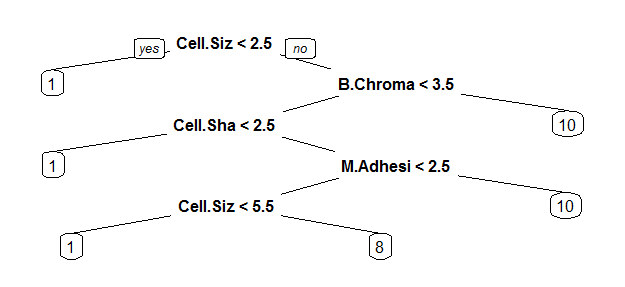
\includegraphics[scale=0.5]{dtreenas.png}
\\This model was used to predict the missing values and the missing values are as follows,
\begin{verbatim}
delmstar[,c(1,7)]
        SCN B.Nuclei
24  1057013        1
41  1096800       10
140 1183246        1
146 1184840        1
159 1193683        1
165 1197510        1
236 1241232        1
250  169356        1
276  432809        1
293  563649       10
295  606140        1
298   61634        1
316  704168       10
322  733639        1
412 1238464        1
618 1057067        1
\end{verbatim}
\end{enumerate}
\end{enumerate}
Answers to the exercises:
\begin{enumerate}
\item Significance of the missing data
\begin{enumerate}
\item Yes, the amount of missing data is significant. From the training data, a correlation matrix was devised which indicates clearly that the B.Nuclei, of which there were missing data has good corelation to the predicted value.\\
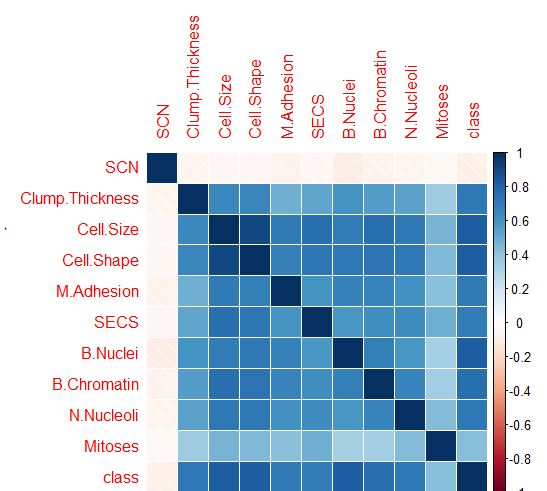
\includegraphics[scale=0.5]{cordelm.jpg}\\
Moreover a decision tree was built over the test data to predict the class, it is seen that several node decisions were taken based on the values of B.Nuclei. Incase if this data is absent, this would lead to increase in entropy at the root level before leaves and the eventual uncertainty of how to split this node.\\
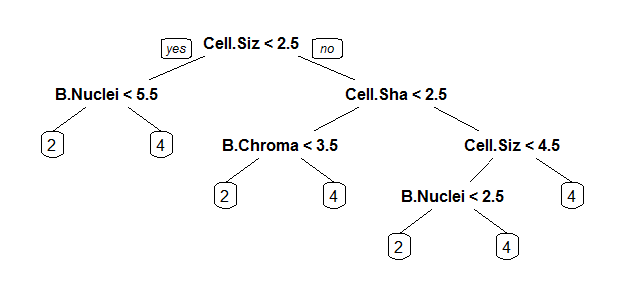
\includegraphics[scale=0.5]{dtreetotal.png}
\end{enumerate}
\item When the tuples are removed because of the missing values, this requires that all these subjects then undergo biopsies again. This would increase the cost. Whereas keeping the tuples with missing values and replacing the old values, we include these tuples to further analysis, and now only 3 people of the missing values require masectomy. Thus this approach reduces both cost and morbidity. 
\end{enumerate}
\item
\begin{enumerate}
\item 
\begin{lstlisting}[language=R]
#Function for Variance
data.variance <- function(dataframe,attributelist){
  names<-colnames(dataframe)
  toPrintnames=c()
  toPrintVal=c()
  for(i in attributelist){
    variance<-var(dataframe[,i])
    toPrintnames=c(toPrintnames,names[i])
    toPrintVal=c(toPrintVal,variance)
  }
  printdf<-as.data.frame(cbind(toPrintnames,toPrintVal))
  colnames(printdf)<-c("label","variance")
  print(printdf)
}
data.variance(delstar,c(2:10))
\end{lstlisting}
The Output of the above code is as follows,\\
\begin{verbatim}
data.variance(delstar,c(2:10))
            label         variance
1 Clump.Thickness 7.95669441784777
2       Cell.Size 9.39511298695165
3      Cell.Shape 8.93161530766027
4      M.Adhesion 8.20571654293848
5            SECS 4.94210894664302
6        B.Nuclei 13.2776950060755
7     B.Chromatin 6.00101329738131
8      N.Nucleoli 9.31877219271542
9         Mitoses 3.00215969738475
\end{verbatim}
It is clearly seen that B.Nuclei has the highest variance
\item Entropy:
\begin{lstlisting}[language=R]
#Function for Entropy
data.entropy <- function(dataframe,attributelist){
  names<-colnames(dataframe)
  toPrintnames=c()
  toPrintVal=c()
  for(i in attributelist){
    entropy_d<-entropy(dataframe[,i],unit="log2")
    toPrintnames=c(toPrintnames,names[i])
    toPrintVal=c(toPrintVal,entropy_d)
  }
  printdf<-as.data.frame(cbind(toPrintnames,toPrintVal))
  colnames(printdf)<-c("label","Entropy")
  print(printdf)
}
data.entropy(delstar,c(2:10))
\end{lstlisting}
The output is,
\begin{verbatim}
data.entropy(delstar,c(2:10))
            label          Entropy
1 Clump.Thickness 9.12010690808455
2       Cell.Size 8.83190208479647
3      Cell.Shape 8.87057622257544
4      M.Adhesion 8.82394225367755
5            SECS 9.13824665773771
6        B.Nuclei 8.73895611645067
7     B.Chromatin 9.08497909039174
8      N.Nucleoli 8.76060529737097
9         Mitoses 8.93412908252063
\end{verbatim}
As with the previous question, B.Nuclei has the least entropy.
\item For KL distance, the package entropy is used. This has functions to empirically calculate the frequency of the two datasets and then performs KL divergence over that probability function.
\begin{lstlisting}[language=R]
#Calculate KL Distance
calculateKL <- function(dataframe,col1,col2){
  output<-matrix(0,nrow=length(col1),ncol = length(col1))
  for (i in 1:length(col1)){
    for(j in 1:length(col1)){
      #print(i)
      k1<-freqs(dataframe[,i])
      k2<-freqs(dataframe[,j])
      kl<-KL.empirical(k1,k2,unit = "log2")
      output[i,j]<-kl
      
    }
  }
  print(output)
}
delkl<-delstar[,2:10]
col<-1:9
calculateKL(delkl,col,col)
\end{lstlisting}
The KL Distance Values are as follows,
\begin{verbatim}
     [,1] [,2] [,3] [,4] [,5] [,6] [,7] [,8] [,9]
 [1,] 0.00 0.35 0.33 0.46 0.26 0.48 0.30 0.48 0.43
 [2,] 0.33 0.00 0.09 0.30 0.23 0.34 0.24 0.32 0.53
 [3,] 0.31 0.09 0.00 0.32 0.24 0.33 0.25 0.33 0.53
 [4,] 0.45 0.28 0.30 0.00 0.33 0.38 0.32 0.44 0.56
 [5,] 0.28 0.24 0.24 0.35 0.00 0.43 0.23 0.36 0.35
 [6,] 0.44 0.30 0.29 0.39 0.40 0.00 0.34 0.50 0.68
 [7,] 0.30 0.25 0.25 0.31 0.21 0.38 0.00 0.36 0.45
 [8,] 0.45 0.27 0.28 0.43 0.34 0.47 0.33 0.00 0.59
 [9,] 0.49 0.48 0.50 0.55 0.35 0.68 0.48 0.54 0.00
\end{verbatim}
\end{enumerate}
\item K Means Implementation for the medical dataset.
\begin{enumerate}
\item K-Means was implemented with java for this exercise. The entire solution has following stages.
\begin{enumerate}
\item Preprocessing : R and R studio are used for preprocessing. The missing values are removed in R and exported as CSV.
\item DataStructure Framework: EJML, Efficient Java Matrix Library is an open source library for extending matrix data structures to java. This supports loading of CSV files directly as matrix, perform advanced operations like matrix, SVD, and calculate distances. However for the purpose of this assignment, they are just used as data structures and this assignment uses no advanced operation required of these data structures.
\item Data munging for EJML : EJML reads data only as matrix and requires space separation instead of comma separated values. Hence these steps are done manually to replace comma with a space and replace first line with number of rows, columns and the data type. Following is a sneak peak of the file used for this assignment.
\begin{verbatim}
683 11 real
1000025 5 1 1 1 2 1 3 1 1 2
1002945 5 4 4 5 7 10 3 2 1 2
1015425 3 1 1 1 2 2 3 1 1 2
1016277 6 8 8 1 3 4 3 7 1 2
1017023 4 1 1 3 2 1 3 1 1 2
1017122 8 10 10 8 7 10 9 7 1 4

\end{verbatim}
\item Program Invocation: The program takes 6 parameters, input file, distance function, number of clusters, number of iterations, tolerance and featurset. Feature set is an comma separated string which contains index of strings that are to be considered for the clustering. This is useful when we can select only few features as predictor values rather than the entire attribute set. Following is the signature used to execute the data analysis. Currently only Eucledian distance is supported. This rather an provision for further improvement.
\begin{verbatim}
"d:\\bcdata.csv" eucledian 2 5 0.1 1,2,3,4,5,6,7,8,9
\end{verbatim}
\item Interpreting the Results: Following is a snapshot of the output.
\begin{verbatim}
------------------------Iteration 2 ------------------------
Cluster Id : 0
Cluster Centers : Type = dense real , numRows = 1 , numCols = 11
1324572.000   7.167   6.744   6.709   5.684   5.449   7.850   6.056   6.017   2.560

Previous Centers : Type = dense real , numRows = 1 , numCols = 11
1324572.000   7.075   6.427   6.416   5.459   5.290   7.427   5.859   5.792   2.514

Cluster Points[1002945, 1016277, 1017122]
Cluster Internal Indexes[1, 3, 5, -1]

Cluster Id : 1
Cluster Centers : Type = dense real , numRows = 1 , numCols = 11
1347749.000   3.022   1.278   1.394   1.343   2.080   1.301   2.085   1.229   1.105  

Previous Centers : Type = dense real , numRows = 1 , numCols = 11
1347749.000   2.874   1.199   1.308   1.264   2.009   1.231   2.007   1.129   1.061  

Cluster Points[1000025, 1015425, 1017023, 841769]
Cluster Internal Indexes[0, 2, 4, 6, 7, -1]

------------------------Has Converged : Tolerance------------------------
\end{verbatim}
The above is a snapshot of the output. There is an iteration number associated with these centroids. There are current centers and previous centers for every centroid. There is also references to data points associated to that centroid and reference to index of the data points. Also it gives details about if the convergence was by tolerance or iteration.
\item Post processing: The output is then brought back to R for interacting plotting and PPV calculation
\end{enumerate}
\item Application Design: The application mainly consists of two classes, Centroid and kMeans. Centroid class is mainly used as a integrated data structure encompassing multiple array vectors and matrices for holding statuses, values and to holding centroids. the driver class consists of modular functions for processing these centroid objects. These centroids are passes as array of objects using Java Collection framework. It has modular functions for reassigning centroid, calculating distances etc.
\item Effect of varying number of blocks and attributes.
\begin{enumerate}
\item Consider Test Data Set 1: 2 centroids with all feature sets. k-Means algorithm was run for this data set with a default tolerance of 0.1 unless stated otherwise. The data is then imported back to R after the clustering. Histograms are then plotted for actual class(Benign or Malignant) of the points in the cluster.\\
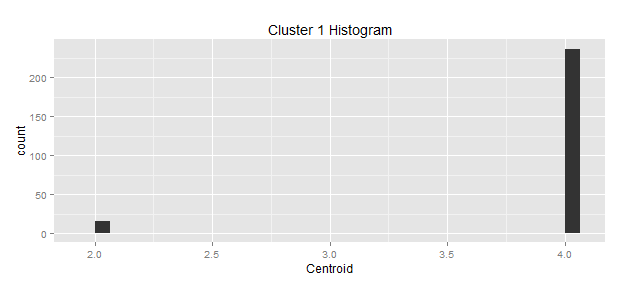
\includegraphics[scale=0.5]{test1_1.png}\\
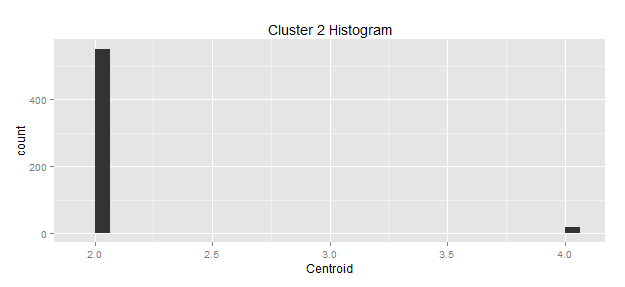
\includegraphics[scale=0.5]{test1_2.png}\\
It can be clearly seen that class 2 is dominant in cluster 2 and class 4 is dominant in cluster 1.
\item Consider Test Data Set 2: Now instead of two Three centroids are calculated.\\
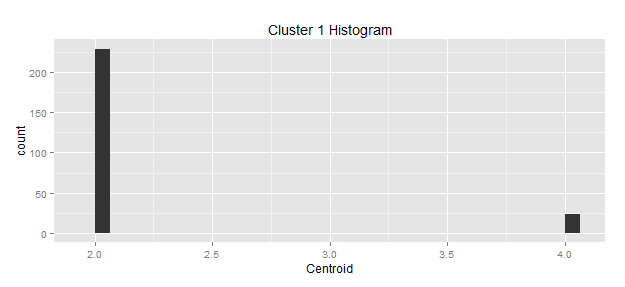
\includegraphics[scale=0.5]{test2_1.png}\\
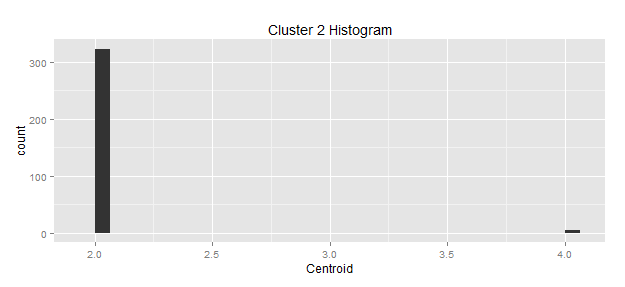
\includegraphics[scale=0.5]{test2_2.png}\\
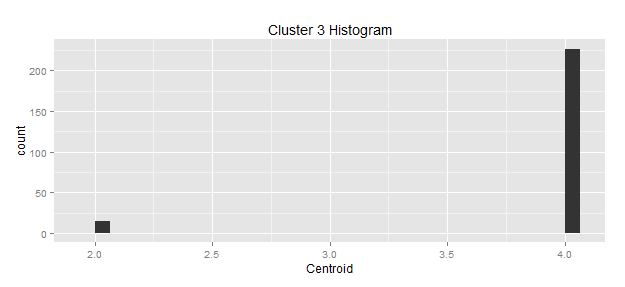
\includegraphics[scale=0.5]{test2_3.png}\\
It can be seen that there are two clusters in which attribute 2 is dominant and the third has attribute 4 dominant.
\item Consider Test Data Set 3 : Consider 4 centroids:\\
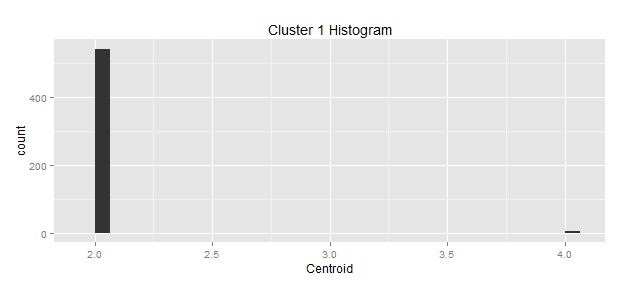
\includegraphics[scale=0.5]{test3_1.png}\\
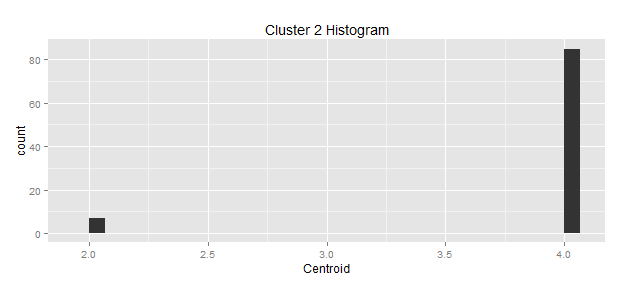
\includegraphics[scale=0.5]{test3_2.png}\\
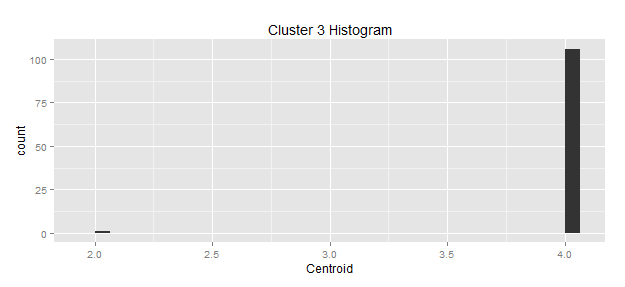
\includegraphics[scale=0.5]{test3_3.png}\\
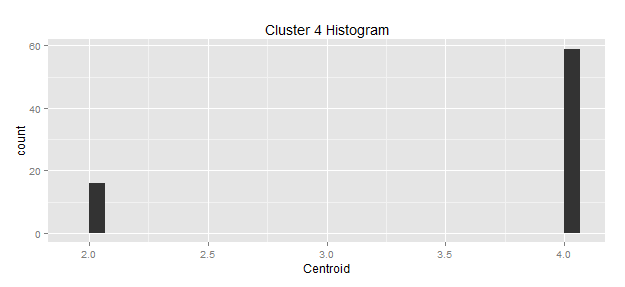
\includegraphics[scale=0.5]{test3_4.png}\\
It can be seen that there are three clusters in which attribute 4 is dominant, whereas in the other cluster attribute 2 is dominant.
\item Hence by intuition, as number of centroid increases the attributes are distributed across the centroids and this is not desired. Hence the best choice at this point is two centroids.
\item Now, changing the feature set, intuitively columns which have higher variance has richer data and might contribute significantly to the predicted value than other attributes. Choosing columns which have top 5 variance, following is the histogram results.\\
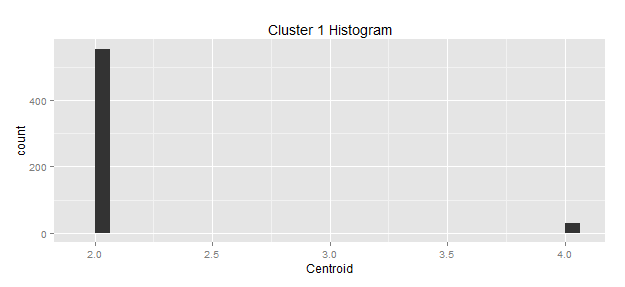
\includegraphics[scale=0.5]{test4_1.png}\\
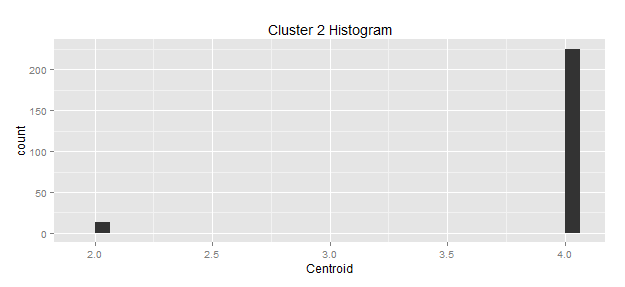
\includegraphics[scale=0.5]{test4_2.png}\\
\begin{verbatim}
data.variance(delstar,c(2:10))
            label         variance
1 Clump.Thickness 7.95669441784777
2       Cell.Size 9.39511298695165
3      Cell.Shape 8.93161530766027
4      M.Adhesion 8.20571654293848
5            SECS 4.94210894664302
6        B.Nuclei 13.2776950060755
7     B.Chromatin 6.00101329738131
8      N.Nucleoli 9.31877219271542
9         Mitoses 3.00215969738475
\end{verbatim}
On Investigation, there were 551 correct and 31 wrong items classified in cluster 1. Cluster 2 had 225 correct items and 13 wrong items.\\ Hence PPV = $\frac{(551+225)}{((551+225)+(13+31))} = 0.9463.$
\item Comparing this to test data 1, which considered all features for calculation of centroid, PPV = $\frac{(225+554)}{(225+554)+(16+19)} = 0.9570025.$. Thus even after reducing half the attributes, there was only a marginal degradation of performance. Hence attributes 2,3,4,6,8 in the above table are good representations of the data. Coincidentally the covariance matrix also infers the same relation.\\
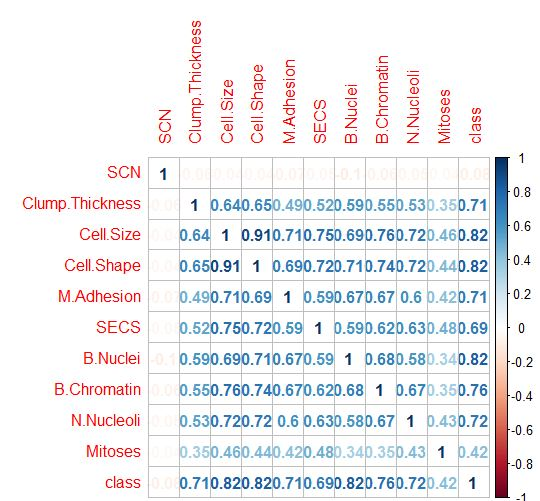
\includegraphics[scale=0.5]{number.jpg}\\
\end{enumerate}
\end{enumerate}
\item Crossfold validations: The data set is divided to 10 parts and K-mean was run on the remaining data. Once we get the centroids to the original data set, a simple distance function call with original centroids and new test data as parameters shall determine the distance of the test data to cluster. Then shortest distance centroid is alloted to that data point and the output is printed. \\
Kmeans program was modified to include the V fold validation. The new additional formal parameters are whether CF validation is required and the test data set location. Eg,
\begin{verbatim}
java -jar KMeansCV.jar "D:\\bcData.csv" eucledian 2 5 0.1 1,2,3,4,5,6,7,8,9 true "C:\\Users\\Ganesh\\Google Drive\\Courses\\CSCI B 565\\Homework\\Homework 2\\test9.csv"
\end{verbatim}
This outputs a little different screen than the previous one. This follows the same line as the previous program, however this at the end predicts the what cluster test data points belongs to.
\begin{verbatim}
------------------------Iteration 2 ------------------------
Cluster Id : 0
Cluster Centers : Type = dense real , numRows = 1 , numCols = 11
1234554.000   3.022   1.278   1.394   1.343   2.080   1.301   2.085   1.229  

Cluster Points[1000025, 1015425,... 841769]
Cluster Id : 1
Cluster Centers : Type = dense real , numRows = 1 , numCols = 11
1224565.000   7.167   6.744   6.709   5.684   5.449   7.850   6.056   6.017  

Cluster Points[1002945, 1016277, 1017122, ...897471]
------------------------Has Converged : Tolerance------------------------
----------Associating Set Data Sets to Calculated Centroid-------
Cluster Id : 0
Cluster Centers : Type = dense real , numRows = 1 , numCols = 11
1234554.000   3.022   1.278   1.394   1.343   2.080   1.301   2.085   1.229  

Cluster Points[1321931, 1321942, 1321942, 1328331, ... 1190546]
Cluster Id : 1
Cluster Centers : Type = dense real , numRows = 1 , numCols = 11
1224565.000   7.167   6.744   6.709   5.684   5.449   7.850   6.056   6.017  

Cluster Points[1331412, 1343068, 1343374, ..., 1190386]

\end{verbatim}
The cluster points at the end give the data points in that cluster.\\ \\
Inorder to determine where this data belongs to, a lookup function is written in R.
\begin{lstlisting}[language=R]
findClass<-function(df,c,label){
  i=length(c)
  a=c()
  for(i in c){
    a=c(a,df[which(df$SCN==i),11])
  }
  #print(a)
  qplot(a,main=label,xlab="Centroid")
  print(length(a[a==2]))
  print(length(a[a==4]))
}
C1=c(1002945, 1016277, 1017122, 1044572, 1050670, ..., 1118039, 1120559)

findClass(delstar,C1,"Cluster 1 Histogram")
[1] 2
[1] 27
\end{lstlisting}
Here the cluster points outputted by the kMeansCV program is used as input to this program. This looks up whether the SCN given belongs to which class. In an example shown above there are 27 correctly classified values and 2 wrong values. This was calculated 10 times for 10 splits of the dataset
\end{enumerate}
\end{document}
